Die bisherige Herangehensweise, den Niederschlag über das Jahresmittel zu Evaluieren ist nicht hinreichend genau. Dadurch wird die lokale und vor allem zeitliche Varianz zu stark beeinträchtigt. Bezieht man hingegen das 99. Quantil der Daten wird die in \ref{sec:zusammenfassung_01} angesprochene tägliche Inkonsistenz umgangen. Das 99. Quantil der Niederschläge entspricht den stärksten örtlichen Regenereignissen. D.Maraun bespricht im Paper \cite{biasMaraun} eine Herangehensweise, in der auch noch die Daten zuvor in die Jahreszeiten aufgeteilt werden, da die Starkregen je nach Jahreszeit unterschiedlichst ausfallen und unterschiedliche Trigger-Mechanismen haben. Im nächsten Kapitel wird zunächst aber das 99. Quantil des gesamten Jahres betrachtet, um einen Vergleichswert zu haben.
\section{Herangehensweise}
\begin{itemize}
	\item Berechnung des 99. jährlichen Quantils aller Datensätze
	\item Vergleichen dieses Quantils mit dem Quantil der Beobachtungsdaten.
	\item Zur Besseren Darstellung Mitteln über die Differenzen aller Jahre
\end{itemize}

\section{Differenzen des 99. Quantils}
Von den Datensätzen (historical, evaluation und APGD) wurden zunächst das jährliche 99. Quantil berechnet. Von den Modelldaten wurden wie in Kapitel \ref{chap:mean} die Beobachtungsdaten abgezogen. Um eine einfachere Darstellung der Ergebnisse zu gewährleisten wurde über Differenzen aller Jahre gemittelt. Daraus ergab sich die Grafik in Abb. \ref{fig:quantile_all}. \\
Wie darin zu erkennen ist, ist im Mittel der Datensatz aus dem regionalen Konvektion-erlaubenden Klimamodell (ALP-3) etwas akkurater in der Simulation der Regenmenge, die bei Starkregenereignissen fällt als die vergleichbaren Datensätze aus dem Modell CLMcom-CCLM4-8-17 (EUR-11). Für alle Datensätze gilt jedoch, dass Starkregenereignisse eher stark unterschätzt als überschätzt werden. Dies erkennt man am stark linkslastigen Verlauf der Kurve, die für alle Datensätze ähnlich verläuft. Doch sie erreichen ihren Peak näher oder weniger nahe bei $0$. Um dieses Ergebnis zu unterstreichen wurden noch die dazugehörigen Boxplots in Abb.\ref{fig:quantile_all_boxplots} abgebildet: Man erkennt, dass alle Biases ziemlich gut bei $0$ liegen, nur der Datensatz Historical von ALP-3 scheint viele Extremniederschläge zu stark zu überschätzen, was sich in einem Bias von $+5.35383 \frac{mm}{Tag}$ zeigt. Das spricht wiederum für ein overfitting des Modells CORDEX FPS-CPS (ALP-3), wie bereits in Kapitel \ref{section:2002} angemerkt wurde. Das erkennt man vor allem beim Boxplot in Abb.\ref{fig:quantile_all_boxplots} für den Evaluation-Datensatz aus ALP-3, der überdurchschnittlich viele Ausreißer darstellt. \\
Dieses im Gemittelten abgezeichnete Verhalten zeigt sich über alle Jahre hinweg, wie bei Betrachten der Grafiken in Abb.\ref{fig:quantile_all_boxplot_all_years_1} \& \ref{fig:quantile_all_boxplot_all_years_2} nachvollzogen werden kann: Die Aufteilung bzw. Streuung der Daten scheint den gemittelten Verlauf abzubilden, ohne große Ausreißer darzustellen. Deshalb wurde daraus geschlossen, dass das Mitteln nicht viel der Variabilität gekostet hat. Somit reicht die Darstellung der gemittelten Daten aus, um diese Besonderheiten des Modells abzubilden.\\
Die Grafiken von Abb.\ref{fig:quantile_alp3}\& \ref{fig:quantile_alp3_1} geben Aufschluss darüber, welche örtlichen Maximalstellen die Abweichung hat. Beachtenswert ist, dass sich die maximalen Abweichungen nun auf drei Hauptspots reduzieren, welche im Südwesten des Alpenhauptkamms, bei Genua und an der Italienisch-Slowenischen Grenze liegen. Dort scheint oft zu wenig Niederschlagsmenge bei Starkregen simuliert bzw. abgebildet worden zu sein. Sehr auffallend ist auch, dass im Evaluation-Datensatz ein Starkregenereignis dauernd überschätzt wird, welches im Süden von Kroatien liegt. Dies scheint wohl ein Ausreißer zu sein, da Mengen von bis zu $500 \frac{mm}{Tag}$ über-simuliert werden.\\

\begin{figure}
	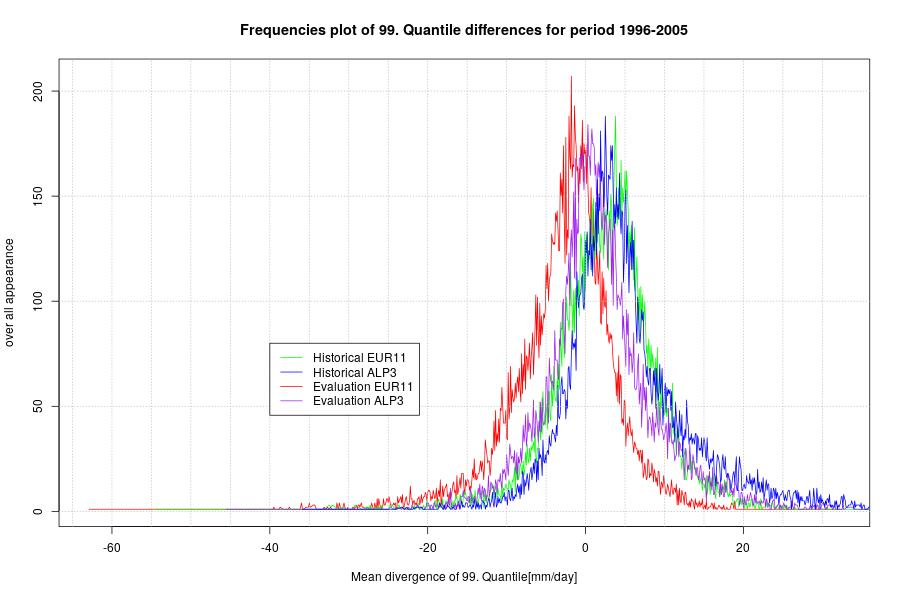
\includegraphics[width=\textwidth]{quantile_all/freq_mean_q99.jpg}
	\caption{Die Abweichungen vom 99. Quantil des Niederschlags, gemittelt über alle Jahre. Der Bereich von $-60\frac{mm}{Tag}$ abwärts wurde abgeschnitten, da es sich in diesem Bereich um seltene Ausreißer handelt.}
	\label{fig:quantile_all}
\end{figure}

\begin{figure}
	\begin{subfigure}{0.49\textwidth}
		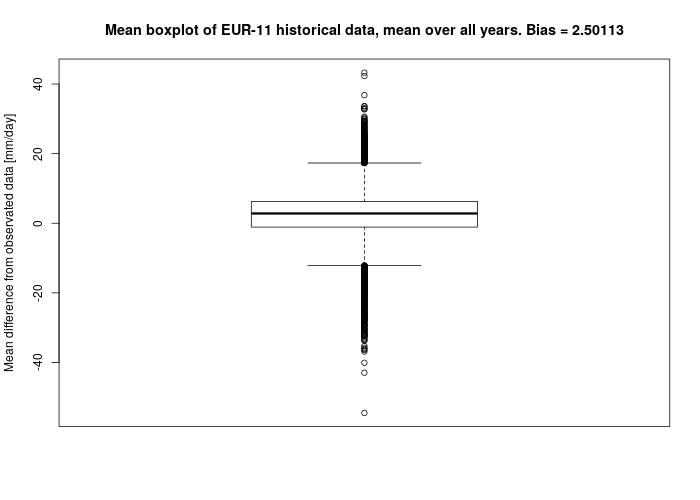
\includegraphics[width=\textwidth]{quantile_all/mean_q99_boxplot_hist_eur11.jpg}
		\caption{EUR-11, Historical}
	\end{subfigure}
	\begin{subfigure}{0.49\textwidth}
		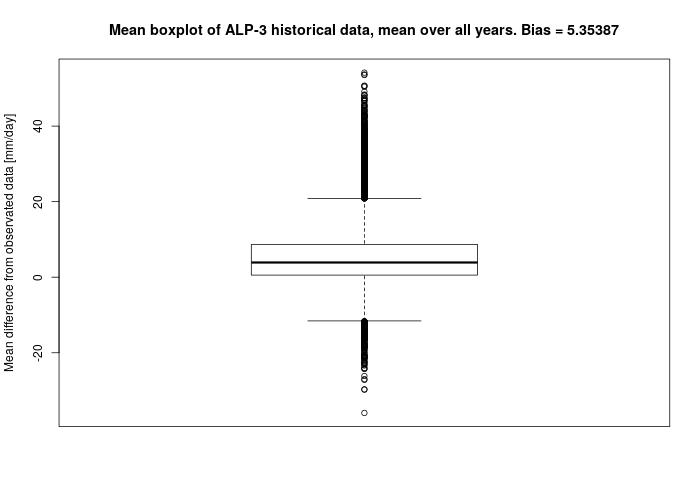
\includegraphics[width=\textwidth]{quantile_all/mean_q99_boxplot_hist_alp3.jpg}
		\caption{ALP-3, Historical}
	\end{subfigure}
	\begin{subfigure}{0.49\textwidth}
		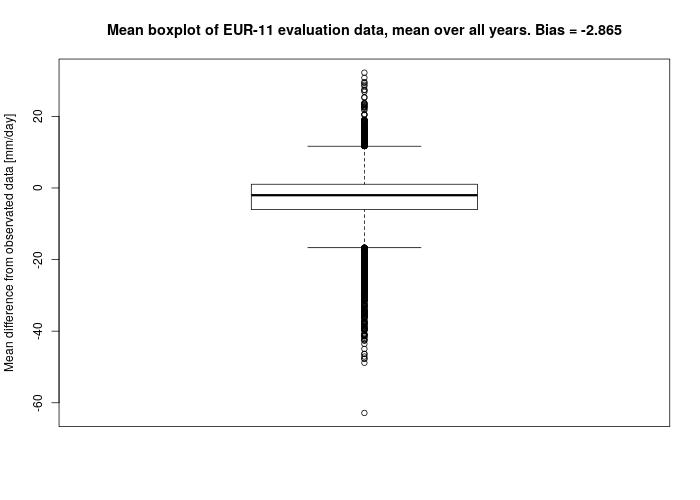
\includegraphics[width=\textwidth]{quantile_all/mean_q99_boxplot_eval_eur11.jpg}
		\caption{EUR-11, Evaluation}
	\end{subfigure}
	\begin{subfigure}{0.49\textwidth}
		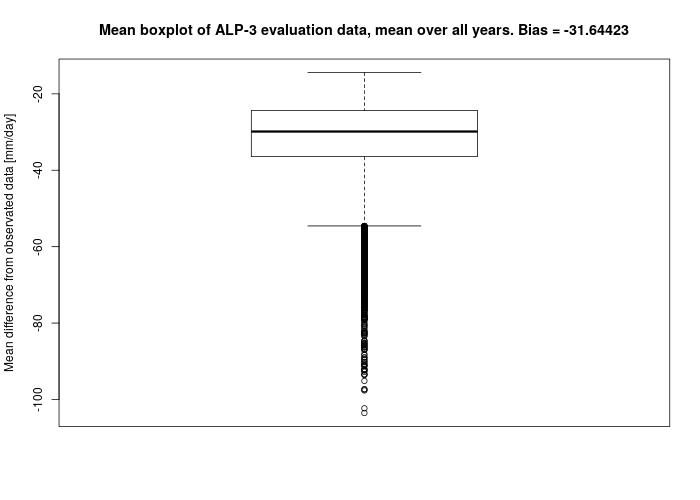
\includegraphics[width=\textwidth]{quantile_all/mean_q99_boxplot_eval_alp3.jpg}
		\caption{ALP-3, Evaluation}
	\end{subfigure}
	\caption{Boxplots der Abweichungen im 99. Quantil, gemittelt über alle Jahre für die 4 Datensätze.}
	\label{fig:quantile_all_boxplots}
\end{figure}

\begin{figure}
	\begin{subfigure}{0.32\textwidth}
		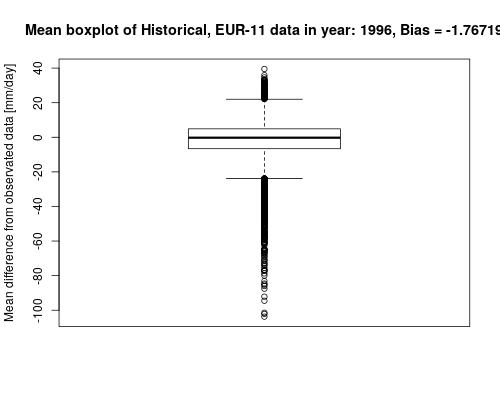
\includegraphics[width=\textwidth]{quantile_all/boxplot_hist_eur11_1996.jpg}
		\caption{Historical, EUR-11, 1996}
	\end{subfigure}
	\begin{subfigure}{0.32\textwidth}
		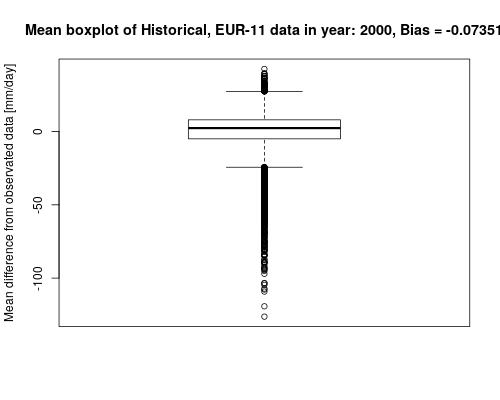
\includegraphics[width=\textwidth]{quantile_all/boxplot_hist_eur11_2000.jpg}
		\caption{Historical, EUR-11, 2000}
	\end{subfigure}
	\begin{subfigure}{0.32\textwidth}
		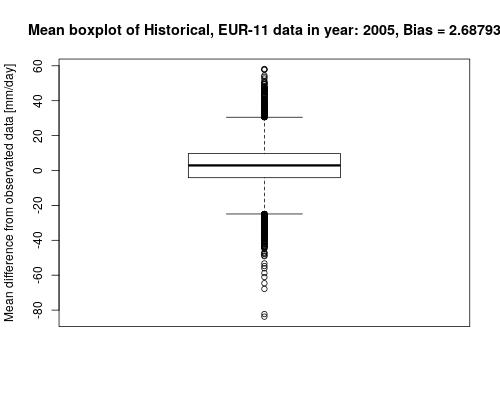
\includegraphics[width=\textwidth]{quantile_all/boxplot_hist_eur11_2005.jpg}
		\caption{Historical, EUR-11, 2005}
	\end{subfigure}
	\begin{subfigure}{0.32\textwidth}
		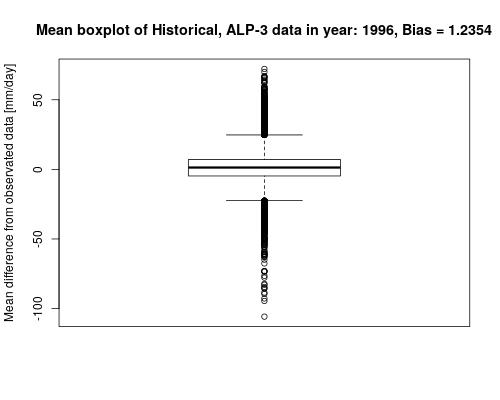
\includegraphics[width=\textwidth]{quantile_all/boxplot_hist_alp3_1996.jpg}
		\caption{Historical, ALP-3, 1996}
	\end{subfigure}
	\begin{subfigure}{0.32\textwidth}
		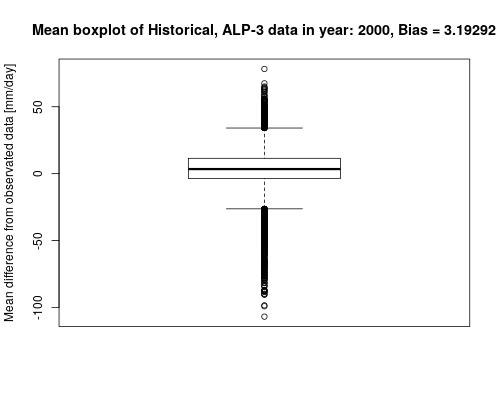
\includegraphics[width=\textwidth]{quantile_all/boxplot_hist_alp3_2000.jpg}
		\caption{Historical, ALP-3, 2000}
	\end{subfigure}
	\begin{subfigure}{0.32\textwidth}
		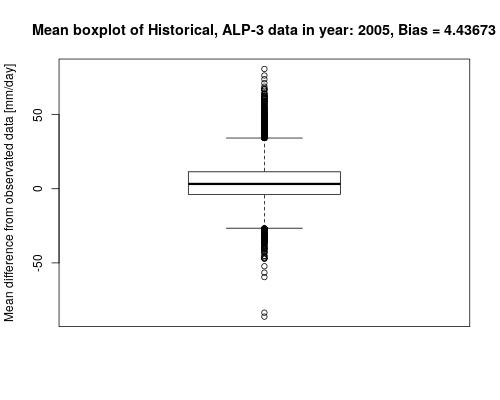
\includegraphics[width=\textwidth]{quantile_all/boxplot_hist_alp3_2005.jpg}
		\caption{Historical, ALP-3, 2005}
	\end{subfigure}
	\caption{Boxplot der Differenzen im 99. Quantil für die Jahre 1996, 2000 und 2005}
\label{fig:quantile_all_boxplot_all_years_1}
\end{figure}

\begin{figure}
	\begin{subfigure}{0.32\textwidth}
		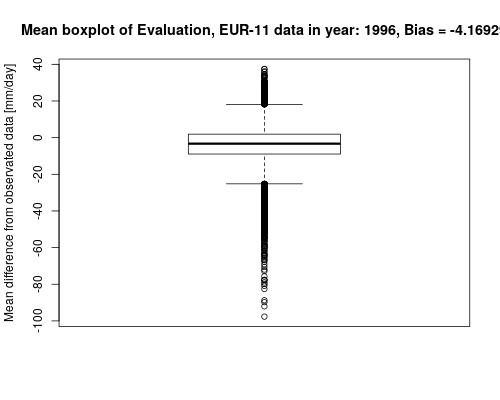
\includegraphics[width=\textwidth]{quantile_all/boxplot_eval_eur11_1996.jpg}
		\caption{Evaluation, EUR-11, 1996}
	\end{subfigure}
	\begin{subfigure}{0.32\textwidth}
		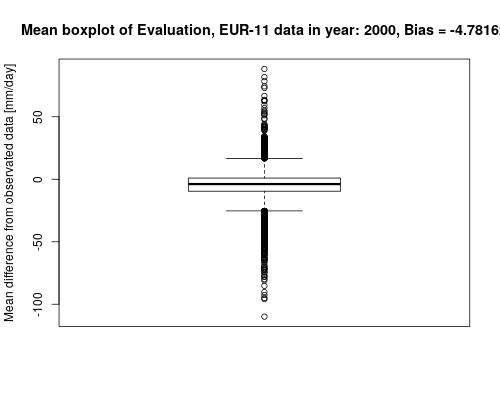
\includegraphics[width=\textwidth]{quantile_all/boxplot_eval_eur11_2000.jpg}
		\caption{Evaluation, EUR-11, 2000}
	\end{subfigure}
	\begin{subfigure}{0.32\textwidth}
		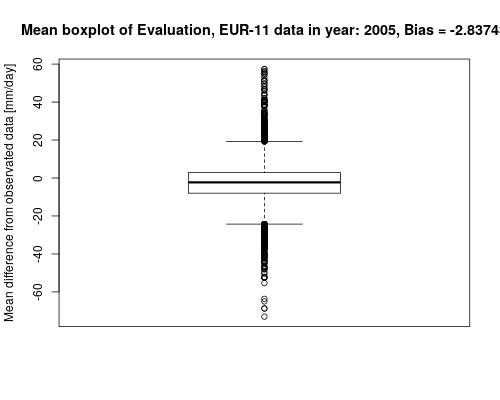
\includegraphics[width=\textwidth]{quantile_all/boxplot_eval_eur11_2005.jpg}
		\caption{Evaluation, EUR-11, 2005}
	\end{subfigure}
	\begin{subfigure}{0.32\textwidth}
		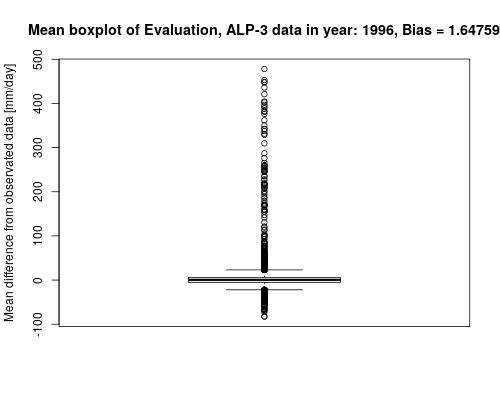
\includegraphics[width=\textwidth]{quantile_all/boxplot_eval_alp3_1996.jpg}
		\caption{Evaluation, ALP-3, 1996}
	\end{subfigure}
	\begin{subfigure}{0.32\textwidth}
		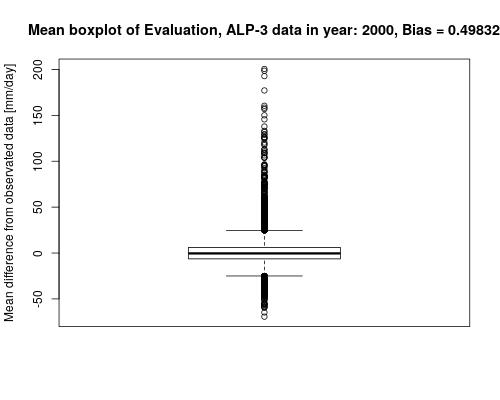
\includegraphics[width=\textwidth]{quantile_all/boxplot_eval_alp3_2000.jpg}
		\caption{Evaluation, ALP-3, 2000}
	\end{subfigure}
	\begin{subfigure}{0.32\textwidth}
		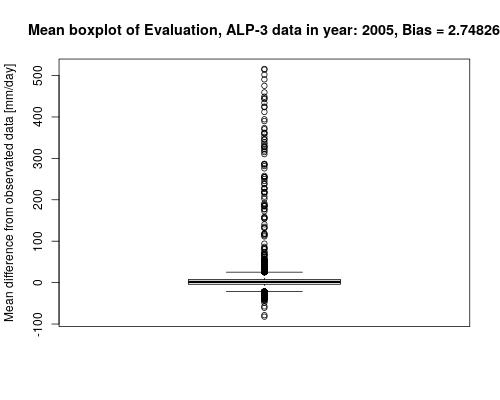
\includegraphics[width=\textwidth]{quantile_all/boxplot_eval_alp3_2005.jpg}
		\caption{Evaluation, ALP-3, 2005}
	\end{subfigure}
	\caption{Boxplot der Differenzen im 99. Quantil für die Jahre 1996, 2000 und 2005}
	\label{fig:quantile_all_boxplot_all_years_2}
\end{figure}

\begin{figure}
	\begin{subfigure}{0.32\textwidth}
		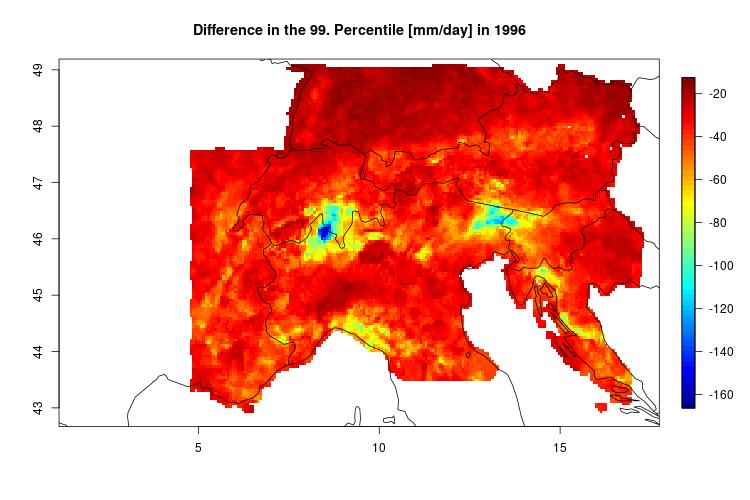
\includegraphics[width=\textwidth]{quantile_all/1996dif_q99_hist_eur11.jpg}
		\caption{Historical, EUR-11, 1996}
	\end{subfigure}
	\begin{subfigure}{0.32\textwidth}
		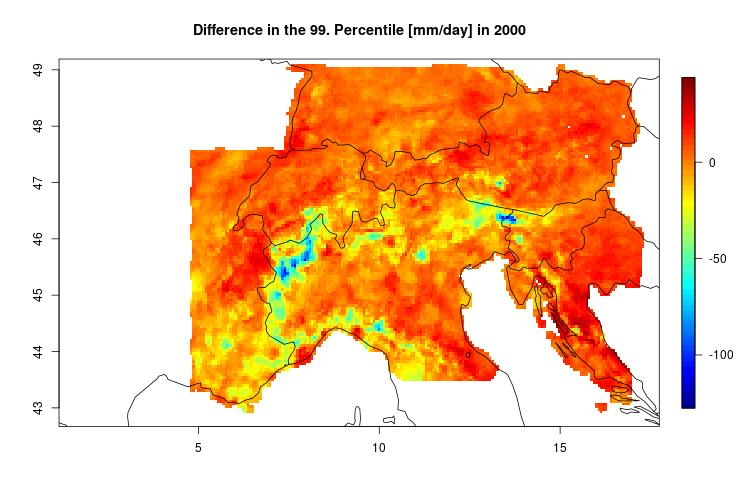
\includegraphics[width=\textwidth]{quantile_all/2000dif_q99_hist_eur11.jpg}
		\caption{Historical, EUR-11, 2000}
	\end{subfigure}
	\begin{subfigure}{0.32\textwidth}
		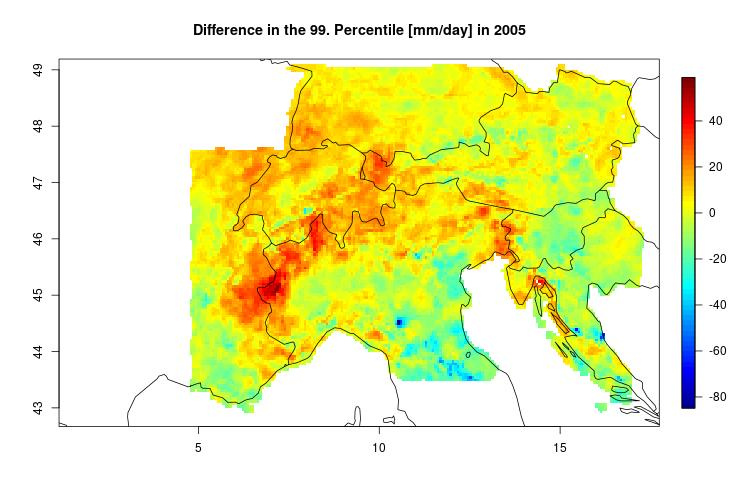
\includegraphics[width=\textwidth]{quantile_all/2005dif_q99_hist_eur11.jpg}
		\caption{Historical, EUR-11, 2005}
	\end{subfigure}
	\begin{subfigure}{0.32\textwidth}
		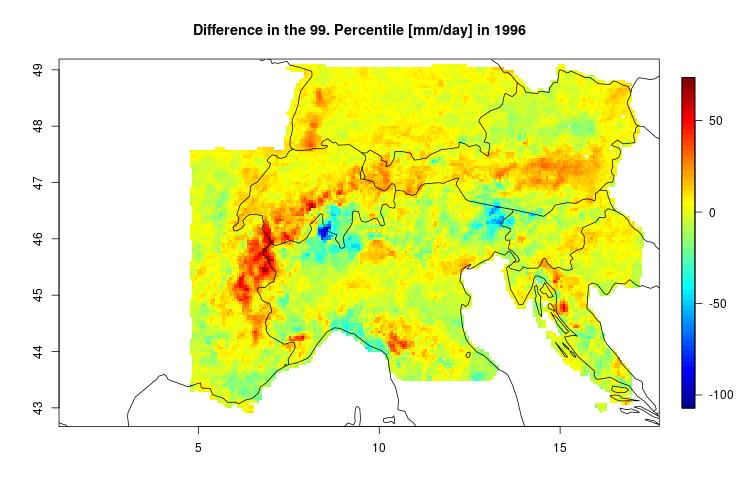
\includegraphics[width=\textwidth]{quantile_all/1996dif_q99_hist_alp3.jpg}
		\caption{Historical, ALP-3, 1996}
	\end{subfigure}
	\begin{subfigure}{0.32\textwidth}
		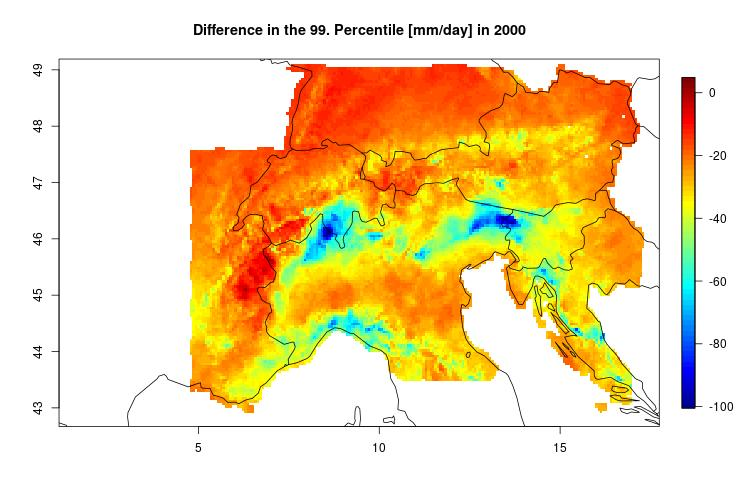
\includegraphics[width=\textwidth]{quantile_all/2000dif_q99_hist_alp3.jpg}
		\caption{Historical, ALP-3, 2000}
	\end{subfigure}
	\begin{subfigure}{0.32\textwidth}
		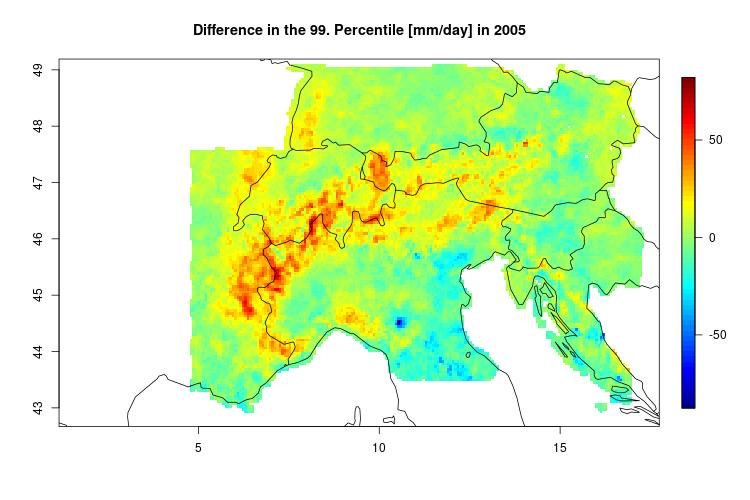
\includegraphics[width=\textwidth]{quantile_all/2005dif_q99_hist_alp3.jpg}
		\caption{Historical, ALP-3, 2005}
	\end{subfigure}
	\caption{Differenzen im 99. Quantil für die Jahre 1996, 2000 und 2005 (gemittelt über das Jahr)}
	\label{fig:quantile_alp3_1}
\end{figure}

\begin{figure}
	\begin{subfigure}{0.32\textwidth}
		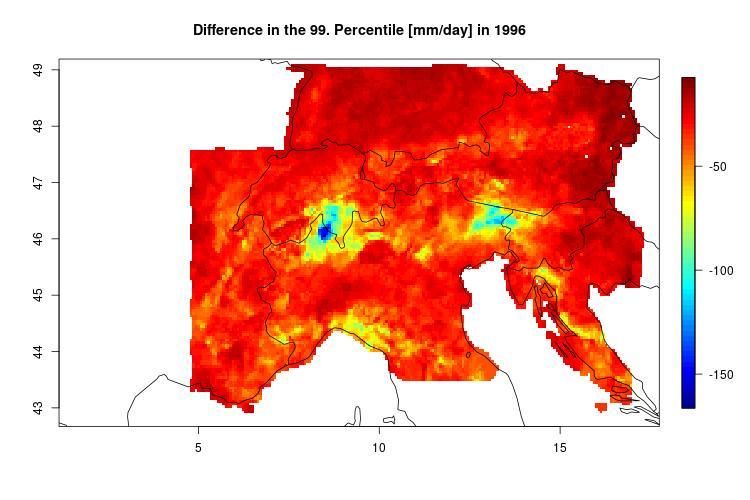
\includegraphics[width=\textwidth]{quantile_all/1996dif_q99_eval_eur11.jpg}
		\caption{Evaluation, EUR-11, 1996}
	\end{subfigure}
	\begin{subfigure}{0.32\textwidth}
		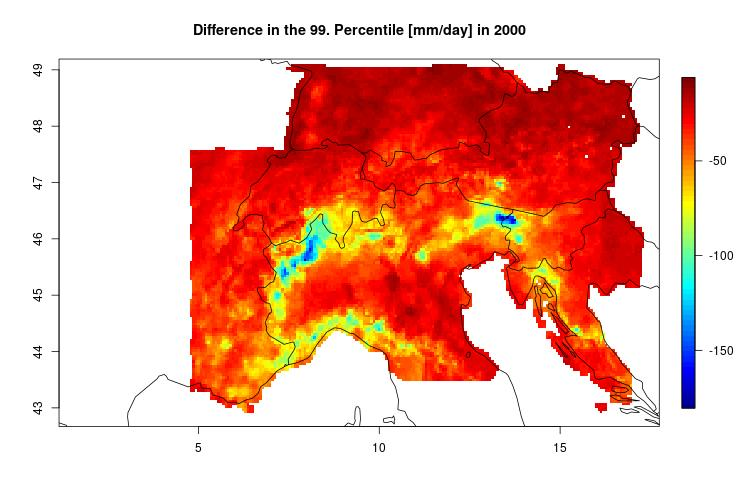
\includegraphics[width=\textwidth]{quantile_all/2000dif_q99_eval_eur11.jpg}
		\caption{Evaluation, EUR-11, 2000}
	\end{subfigure}
	\begin{subfigure}{0.32\textwidth}
		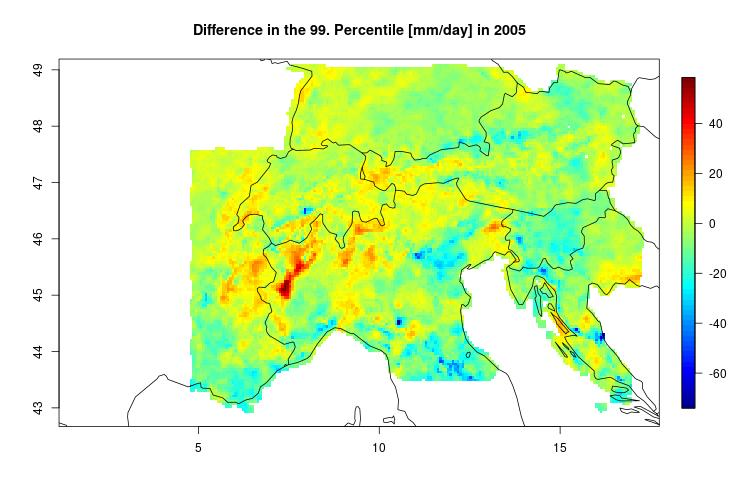
\includegraphics[width=\textwidth]{quantile_all/2005dif_q99_eval_eur11.jpg}
		\caption{Evaluation, EUR-11, 2005}
	\end{subfigure}
	\begin{subfigure}{0.32\textwidth}
		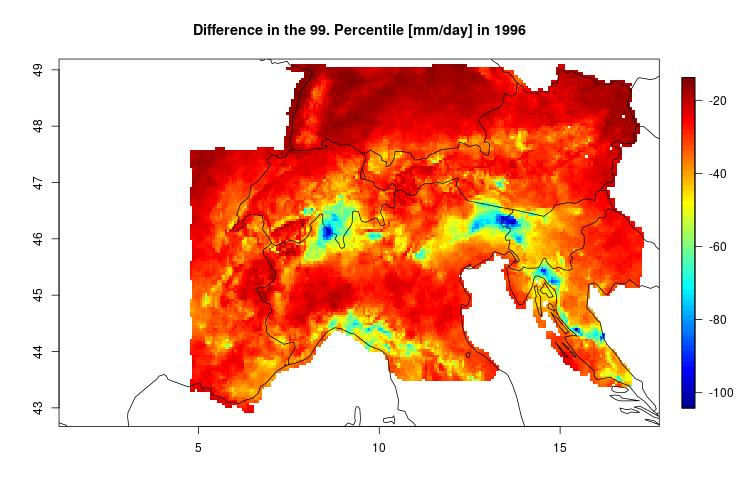
\includegraphics[width=\textwidth]{quantile_all/1996dif_q99_eval_alp3.jpg}
		\caption{Evaluation, ALP-3, 1996}
	\end{subfigure}
	\begin{subfigure}{0.32\textwidth}
		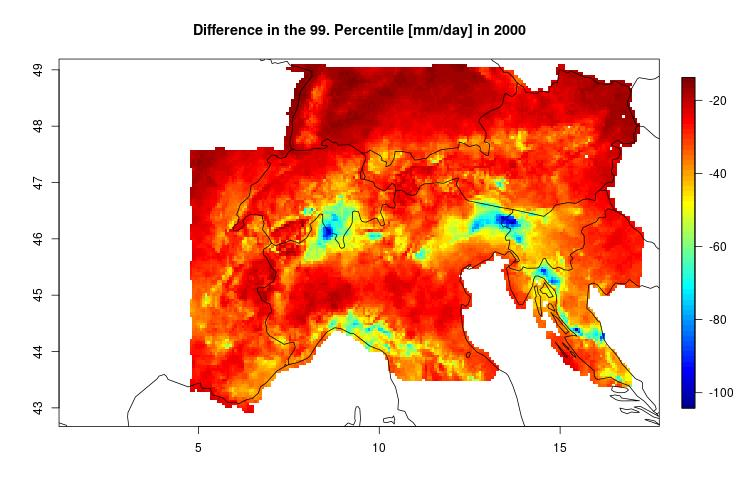
\includegraphics[width=\textwidth]{quantile_all/2000dif_q99_eval_alp3.jpg}
		\caption{Evaluation, ALP-3, 2000}
	\end{subfigure}
	\begin{subfigure}{0.32\textwidth}
		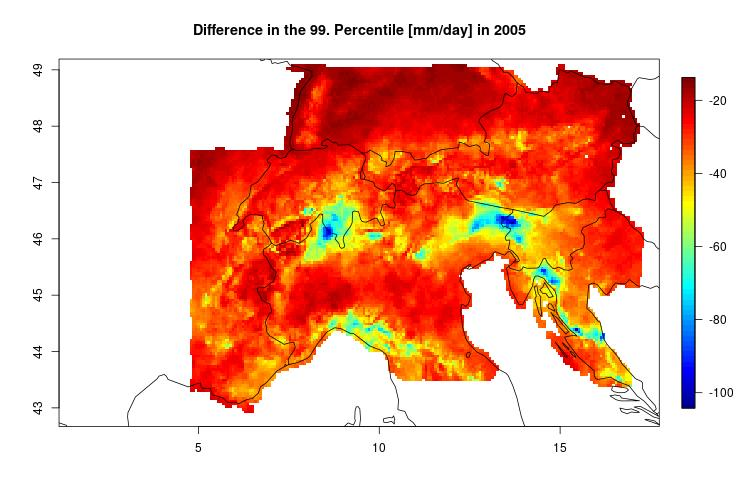
\includegraphics[width=\textwidth]{quantile_all/2005dif_q99_eval_alp3.jpg}
		\caption{Evaluation, ALP-3, 2005}
	\end{subfigure}
	\caption{Differenzen im 99. Quantil für die Jahre 1996, 2000 und 2005 (gemittelt über das Jahr)}
	\label{fig:quantile_alp3}
\end{figure}

\section{Zusammenfassung}
In diesem Kapitel wurden die 99. Quantile und somit die modellierten Starkregenereignisse des gesamten Jahres mit den Beobachtungsdaten verglichen. Dadurch wurde ein guter Aufschluss darüber erlangt, wie die Starkregenereignisse im generellen durch die unterschiedlichen Datensätzen simuliert werden. Wie es scheint, herrscht eine relativ gute Abbildung der tatsächlichen gemessenen Wertem, sieht man von den Ausreißern ab. In den Abbildungen \ref{fig:quantile_alp3} erkennt man gut, dass manche Regionen besonders stark unterschätzte Starkregen-Ereignisse aufweisen: 
\begin{itemize}
	\item Der Bereich rund um Genua
	\item Das Grenzgebiet von Italien zur südlichen Schweiz
	\item Ein Bereich an der Slowenisch-Italienische Grenze
\end{itemize}
Diese Regionen wurden in ''Major flood disasters in Europe: 1950–2005'' \cite{barredo_major_2007} unter anderem als Regionen größerer Flutkatastrophen genannt. Das besonders große Abzeichnen der Differenzen in diesen Regionen weißt darauf hin, dass die Klimasimulation für solche Orte gesondert betrachtet werden muss oder den Modellen noch einige Parameter beziehungsweise Module für solche orthographische und geographischen Konstellationen fehlen.